%
% motivation-definition.tex
%
% (c) 2026 Damien Flury, OST Ostschweizer Fachhochschule
%
% !TEX root = ../../buch.tex
% !TEX encoding = UTF-8
%
\section{Motivation und Definition
\label{hauptwert:section:motivation-definition}}
\kopfrechts{Teil 0}
\subsection{Uneigentliche Integrale}

Man betrachte die Funktion
\begin{equation}
f(x) = \frac{1}{x}
\end{equation}
und damit das Integral
\begin{equation}
\int_{-\infty}^{\infty} f(x)\,dx
= \int_{-\infty}^{\infty} \frac{1}{x}\,dx.
\end{equation}
%
% kehrwert.tex
%
% (c) 2026 Damien Flury, OST Ostschweizer Fachhochschule
%
\begin{figure}
\centering

\includegraphics{papers/hauptwert/images/kehrwert.pdf}
\caption{Graph der Funktion $f(x)=1/x$ mit Polstelle bei $x=0$.
Die schraffierten Flächen zeigen eine unsymmetrische Wahl der
Integrationsgrenzen um die Polstelle.
\label{hauptwert:figure:kehrwert}}
\end{figure}

Abbildung \ref{hauptwert:figure:kehrwert} zeigt den Graphen des Integranden
$f(x)=1/x$.
Beim Lösen dieses Integrals fällt schnell ein Problem auf:
Die Funktion hat bei $x = 0$ eine Polstelle.

\subsection{Ein erster Versuch}
Um das Integral zu lösen, wäre der erste natürliche Schritt,
das Integral an der Polstelle aufzuteilen
und sich ihr mit unabhängigen Grenzwerten zu nähern:
\begin{equation}
\int_{-\infty}^{\infty} f(x)\,dx
= \lim_{\epsilon_1\to 0^+} \int_{-\infty}^{-\epsilon_1} f(x)\,dx
+ \lim_{\epsilon_2\to 0^+} \int_{\epsilon_2}^{\infty} f(x)\,dx.
\label{hauptwert:equation:aufteilung}
\end{equation}
Da auch die Integrationsgrenzen $\pm\infty$ uneigentlich sind,
muss jedes Teilintegral nochmals aufgeteilt
und durch einen eigenen Grenzwert ersetzt werden.
Das rechte Teilintegral wird dazu an einer beliebigen Zwischenstelle
$c > 0$ aufgeteilt:
\begin{equation}
\lim_{\epsilon_2\to 0^+} \int_{\epsilon_2}^{c} \frac{1}{x}\,dx
+ \lim_{R\to\infty} \int_{c}^{R} \frac{1}{x}\,dx
= \underbrace{\lim_{\epsilon_2\to 0^+} \left(\ln c - \ln \epsilon_2\right)}_{+\infty}
+ \underbrace{\lim_{R\to\infty} \left(\ln R - \ln c\right)}_{+\infty}.
\label{hauptwert:equation:rechts}
\end{equation}
Beide Grenzwerte divergieren gegen $+\infty$,
das rechte Teilintegral existiert also nicht.
Aus Symmetriegründen divergiert das linke Teilintegral
genauso gegen $-\infty$.
Die Aufteilung \eqref{hauptwert:equation:aufteilung} führt also auf den
unbestimmten Ausdruck $\infty - \infty$,
das uneigentliche Integral existiert nicht.

\subsection{Der Cauchy-Hauptwert -- Symmetrische Annäherung}
Die zu Grunde liegende Idee vom Cauchy Hauptwert ist, dass
man sich der Polstelle symmetrisch annähert, das heisst mit
einem einzigen, gemeinsamen $\epsilon$ und symmetrischen Grenzen $\pm R$.
%
% kehrwert-symmetrisch.tex
%
% (c) 2026 Damien Flury, OST Ostschweizer Fachhochschule
%
\begin{figure}
\centering
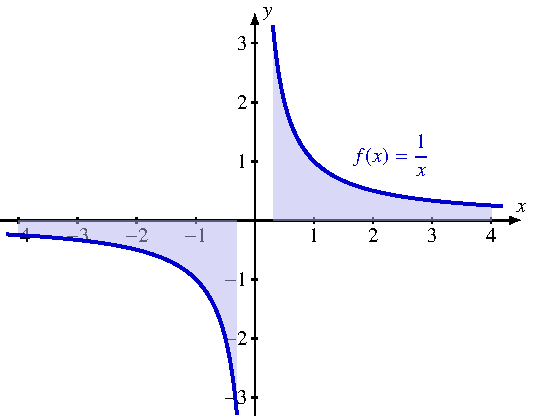
\includegraphics{papers/hauptwert/images/kehrwert-symmetrisch.pdf}
\caption{Graph der Funktion $f(x)=1/x$ mit Polstelle bei $x=0$.
Die schraffierten Flächen zeigen die symmetrische Wahl der
Integrationsgrenzen $\pm\epsilon$ und $\pm R$ um die Polstelle.
\label{hauptwert:figure:kehrwert-symmetrisch}}
\end{figure}

Abbildung \ref{hauptwert:figure:kehrwert-symmetrisch} zeigt diese symmetrische
Wahl der Integrationsgrenzen im Vergleich zur unsymmetrischen Aufteilung
aus Abbildung \ref{hauptwert:figure:kehrwert}.
\begin{equation}
 \int_{-R}^{-\epsilon} \frac{1}{x}\,dx
+ \int_{\epsilon}^{R} \frac{1}{x}\,dx
  = \bigl(\ln\epsilon - \ln R\bigr) + \bigl(\ln R - \ln\epsilon\bigr)
= 0.
\label{hauptwert:equation:symmetrisch}
\end{equation}
Der Grenzwert $\epsilon \to 0^+$, $R \to \infty$ existiert somit und ist $0$,
im Gegensatz zum unabhängigen Grenzwert aus
\eqref{hauptwert:equation:aufteilung}, welcher nicht existiert.
